% \AtBeginSection[]{
%     \begin{frame}
%         \frametitle{}
%         \tableofcontents[currentsection]
%     \end{frame}
% }

%%%%%%%%%%%%%%%%%%%%%%%%%%%%%%%%%%%%

\addtocounter{framenumber}{-2}

\section{Introduction}

\begin{frame}{Introduction}{General context}

    \begin{columns}

        \begin{column}{0.7\textwidth}

            \begin{itemize}
                \item \textbf{Increasing attack surface}
                      \begin{itemize}
                          \item IoT/IoBT: drones, autonomous vehicles
                      \end{itemize}
                \item \textbf{Challenges during attack}
                      \begin{itemize}
                          \item Operators' limitations: time constraints, workload, complexity\dots
                          \item Environment's limitations: jamming, communication interruption\dots
                      \end{itemize}
            \end{itemize}

            \ \\

            $\Longrightarrow$ Need for: \textbf{reactivity, flexibiity, autonomy}\dots

            \begin{itemize}
                \item A Multi-Agent approach for Cyberdefense
                      \begin{itemize}
                          \item An agent\dots
                          \item A Multi-Agent System (MAS)\dots
                      \end{itemize}
            \end{itemize}

            \ \\

            $\Longrightarrow$ Promising for: \textbf{adaptation, scalability, sub-task delegation}\dots

        \end{column}

        \begin{column}{0.4\textwidth}
            \begin{figure}
                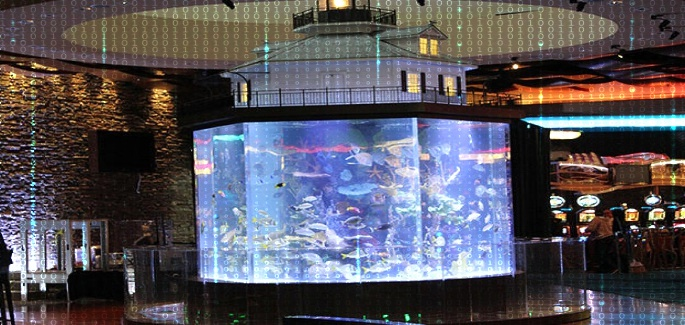
\includegraphics[width=\linewidth]{figures/casino.jpg}
                \caption*{\tiny\url{https://hackread.com/hackers-casinos-fish-tank-smart-thermometer-hack/}}
            \end{figure}

            \vspace{0.cm}

            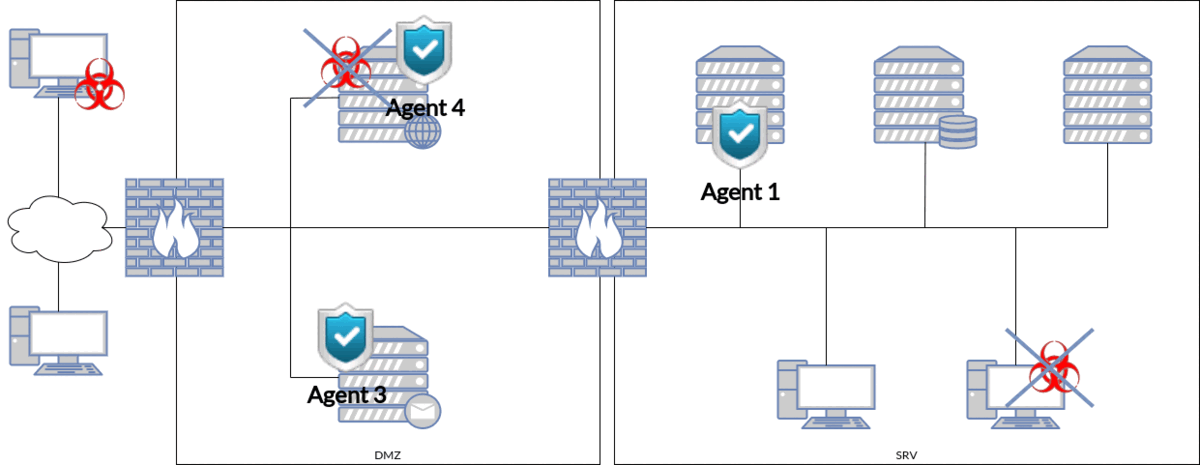
\includegraphics[width=\linewidth]{figures/company_network.png}
        \end{column}

    \end{columns}

\end{frame}

\begin{frame}{Introduction}{General context}

    \begin{columns}

        \begin{column}{0.5\textwidth}

            \begin{itemize}
                \item MASCARA (Multi Agent Centric AICA Reference Architecture)
                      \begin{itemize}
                          \item AICA theorized by “IST-152 NATO” (2016-2019)
                      \end{itemize}

                \item Detect, identify and characterize anomalies/attacks

                      \begin{itemize}
                          \item Plan and execute countermeasures
                      \end{itemize}

                \item Communicate with C2 / operators…

                      \begin{itemize}
                          \item Be autonomous, stealthy, interoperable, capable of learning
                      \end{itemize}

                \item MASCARA: A Multi-Agent vision of AICA
                      \begin{itemize}
                          \item An implicit organization
                      \end{itemize}
            \end{itemize}

        \end{column}

        \hspace{-2ex}
        \begin{column}{0.6\textwidth}
            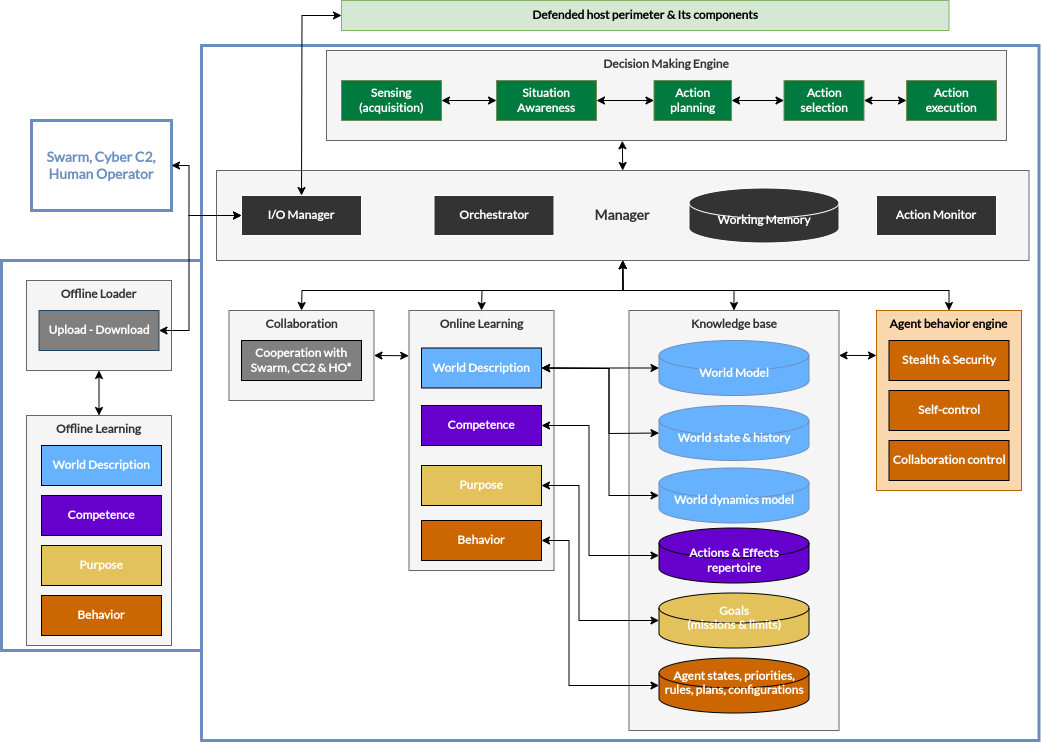
\includegraphics[width=\linewidth]{figures/mascara.png}
        \end{column}

    \end{columns}

\end{frame}

\begin{frame}{Introduction}{Problem}

    \begin{alertblock}{General problem}
        \textbf{What organizational mechanisms of the Cyberdefense MAS (AICA) to optimize its operation taking into account its constraints?}
    \end{alertblock}

    \begin{columns}

        \begin{column}{0.6\textwidth}
            \begin{figure}
                \centering
                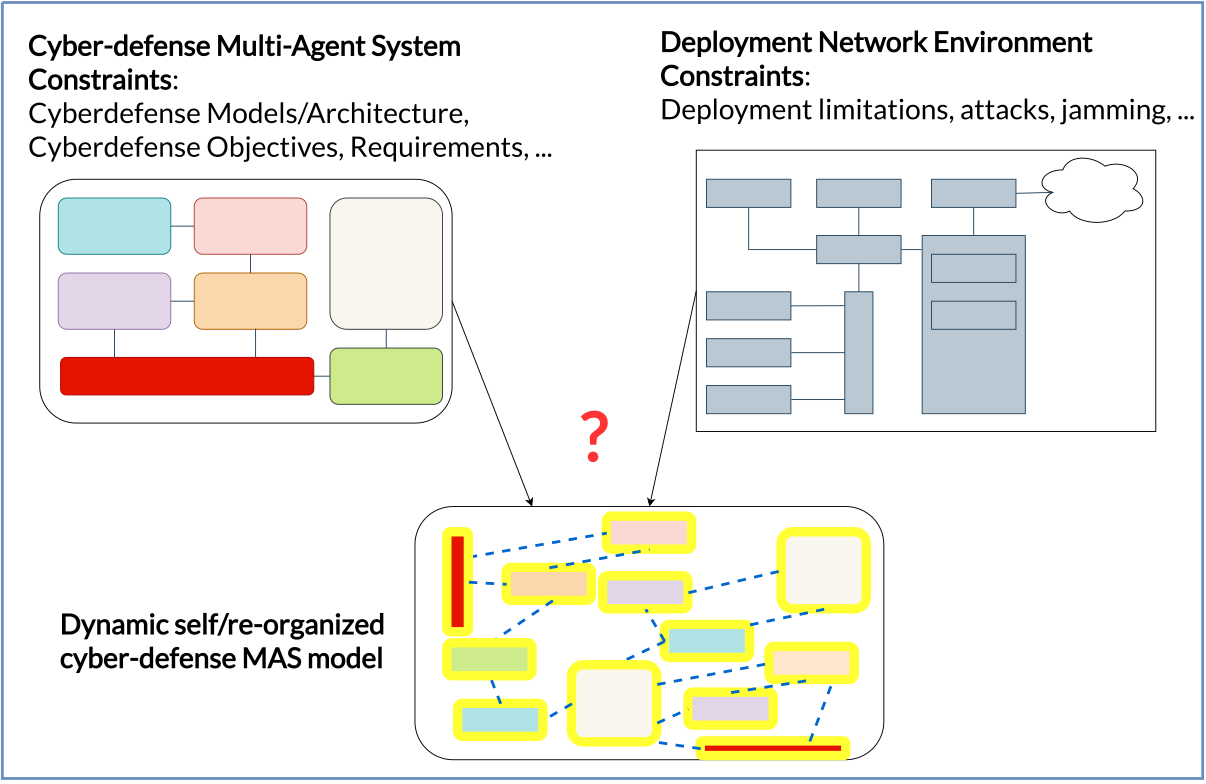
\includegraphics[width=0.95\linewidth]{figures/general_problem_illustration.png}
            \end{figure}
        \end{column}

        \begin{column}{0.5\textwidth}
            \textbf{Literature study of available Cyberdefense MAS (CMAS) organizations}

            \begin{itemize}
                \item Few works dealing with a Multi-Agent approach to Cyberdefense
                \item Difficult to have a general vision of the effects of the organizations involved depending on the deployment environment
            \end{itemize}

            \ \\

            $\Longrightarrow$ \textbf{Need a study framework to address the problem…}
        \end{column}
    \end{columns}

\end{frame}

\begin{frame}{Introduction}{Approach for addressing the problem}

    A methodological contribution:
    \begin{itemize}

        % \item Review of work for the development of Cyberdefense MAS
        %       \begin{itemize}
        %           \item Expectations of a methodology for the development of Cyberdefense MAS
        %           \item Overview of available work versus expectations
        %           \item Discussion on methodological obstacles
        %       \end{itemize}

        \item \textbf{Need for modeling problem \& design foundation}
              \begin{itemize}
                  \item[$\rightarrow$] \textbf{CybMASFM}: Markovian framework + Digital Twins (simulation/emulation coupling)
              \end{itemize}

        \item \textbf{Need for automated safe design}
              \begin{itemize}
                  \item[$\rightarrow$] \textbf{CybMASDA}: Comprehensive design process
                      \begin{itemize}
                          \item[$\rightarrow$] OMARL: MARL + Organizational model
                      \end{itemize}
              \end{itemize}

        \item \textbf{Need for practical design means}
              \begin{itemize}
                  \item[$\rightarrow$] \textbf{CybMASDE}: implemented CybMASDA as an API + GUI
              \end{itemize}

    \end{itemize}

    \ \\
    \begin{itemize}

        \item Academic \& industrial \textbf{case studies} for AICA\dots
              \begin{itemize}
                  \item Drone swarm
                  \item Company Infrastructure
                  \item Kubernetes/Drones environment
              \end{itemize}

    \end{itemize}

\end{frame}

\section{CybMASFM}

\begin{frame}{Cyberdefense Multi-Agent Systems Formal Model}{Overview}

    \begin{columns}

        \hspace{-2ex}

        \begin{column}{0.45\textwidth}

            \begin{figure}
                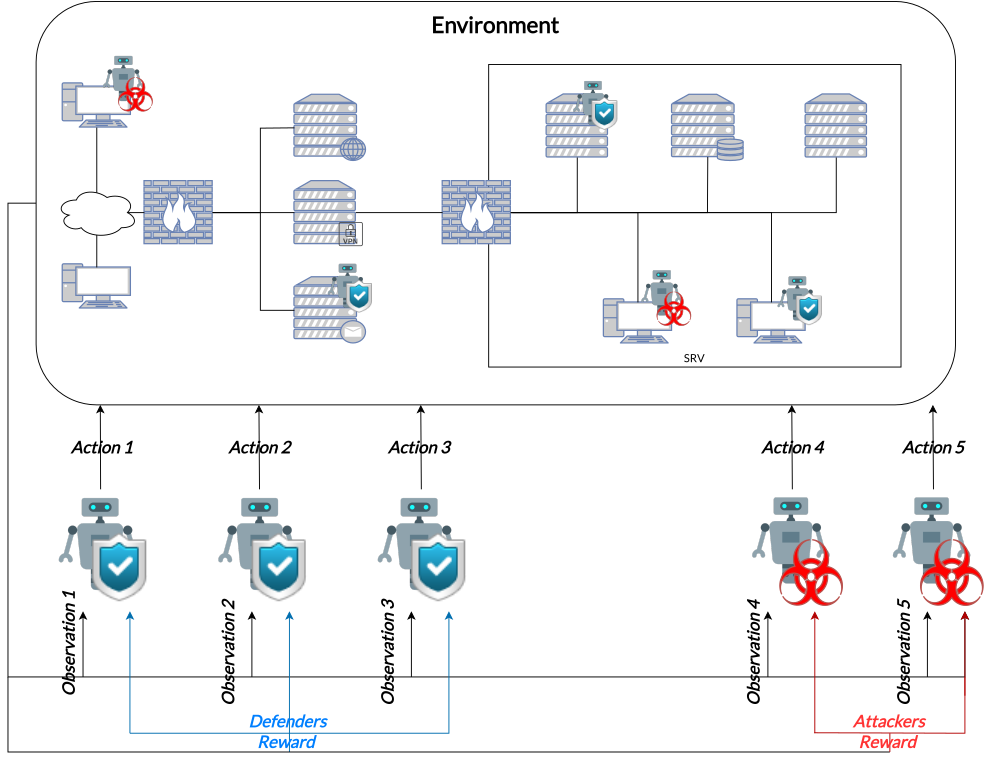
\includegraphics[width=\linewidth]{figures/marl_illustration.png}
            \end{figure}

            {\tiny \begin{spacing}{0.5}
                Soulé, J., Jamont, J.-P., Occello, M., Théron, P., \& Traonouez, L.-M. Towards a Multi-Agent Simulation of Cyber-attackers and Cyber-defenders Battles. IEEE SMC 2023.
            \end{spacing}}

        \end{column}

        \begin{column}{0.65\textwidth}
            \vspace{-2ex}

            \begin{center}
                \begin{minipage}{0.95\linewidth}
                    \centering
                    \begin{block}{Markovian models for MARL: Dec-POMDP}
                        {\small
                            Decentralized Partially Observable Markov Decision Process (Dec-POMDP)~\cite{Oliehoek2016}
                            \begin{itemize}
                                \item considers multiple agents in a similar MAS fashion
                                \item stochastic processes for uncertainty in environmental changes including observations;
                                \item reward function is common to agents which fosters training for collaborative oriented actions~\cite{Beynier2013}
                            \end{itemize}
                        }
                        \

                        { \scriptsize

                        $(S,\{A_i\},T,R,\{\Omega_i\},O,\gamma)$ , where
                        \begin{itemize}
                            \item $S = \{s_1, ..s_{|S|}\}$: The set of the possible states;
                            \item $A_{i} = \{a_{1}^{i},..,a_{|A_{i}|}^{i}\}$: The set of the possible actions for agent $i$;
                            \item $T$ so that $T(s,a,s') = \probP{(s'|s,a)}$ : The set of conditional transition probabilities;
                            \item $R: S \times A \times S \rightarrow \mathbb{R}$: The reward function
                            \item $\Omega_{i} = \{o_{1}^{i},..,o_{|\Omega_{i}|}^{i}\}$: The set of observations for agent $ag_i$;
                            \item $O$ so that $O(s',a,o) = \probP{(o|s',a)}$ : The set of conditional observation probabilities;
                            \item $\gamma \in [0,1]$, the discount factor.
                        \end{itemize}

                        }

                    \end{block}

                \end{minipage}
            \end{center}

        \end{column}

    \end{columns}


\end{frame}

\section{CybMASDA}

\begin{frame}{Cyberdefense Multi-Agent Systems Development Approach}{MAS Design context}

    \begin{figure}
        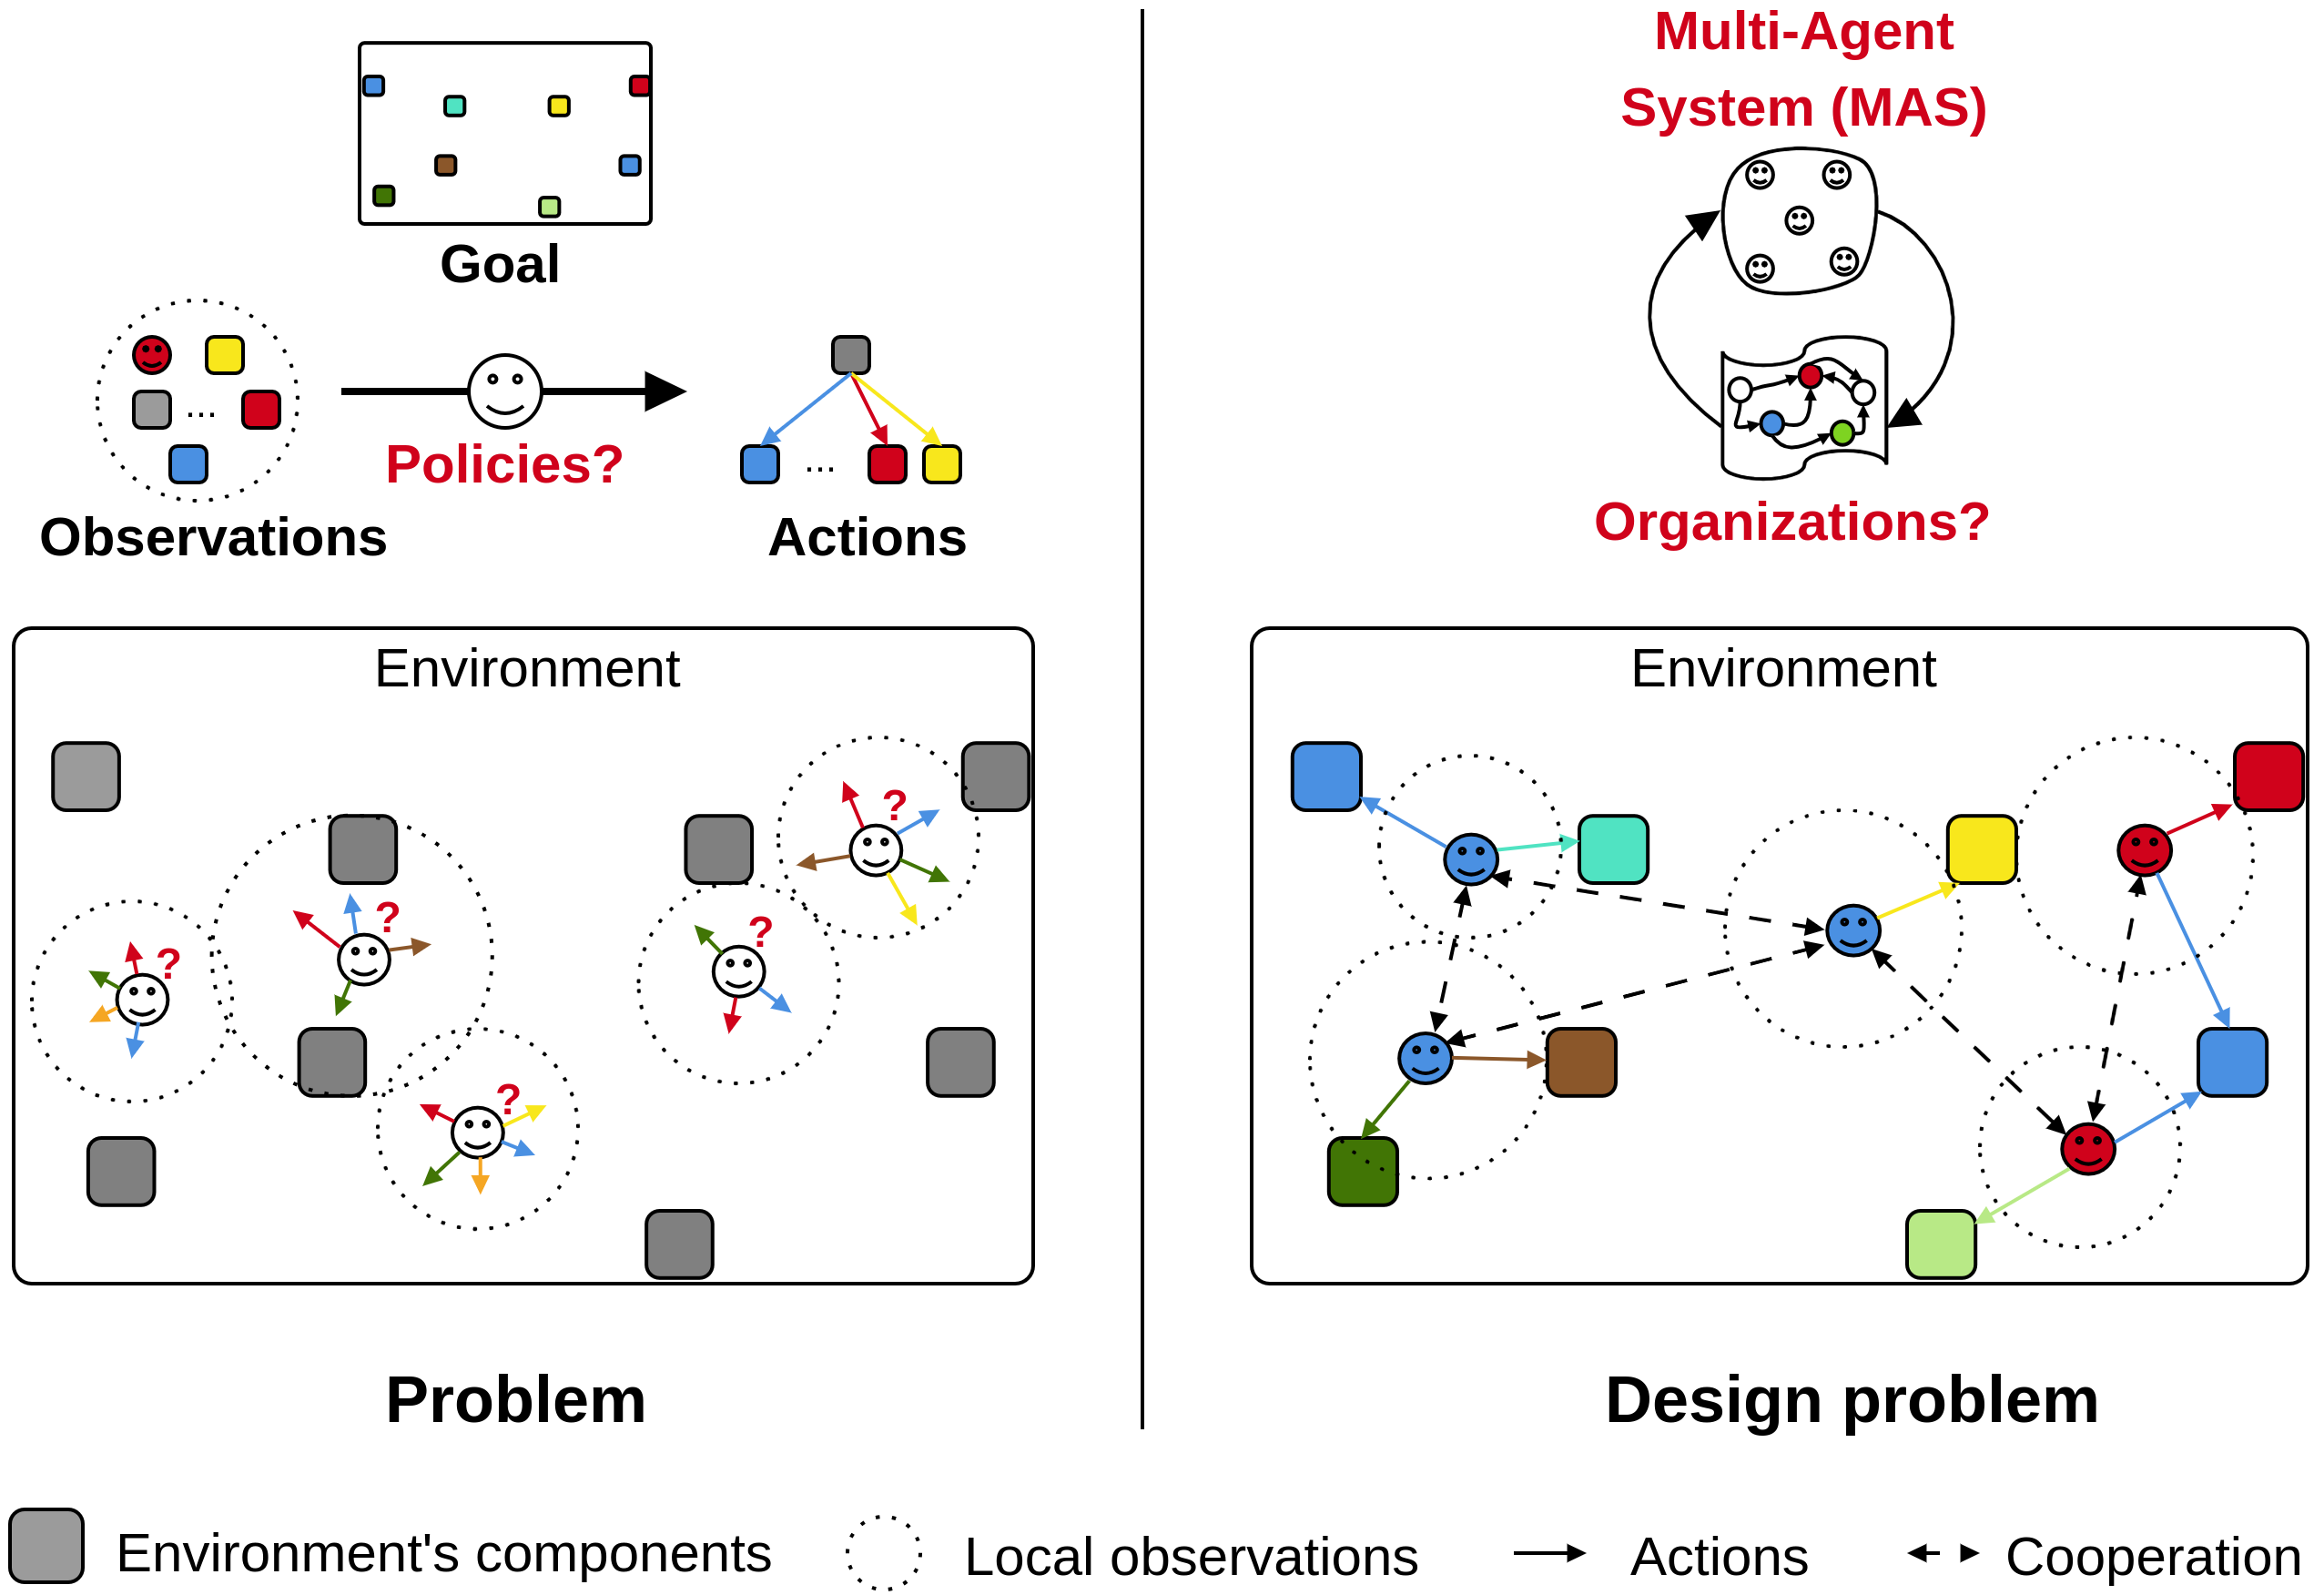
\includegraphics[width=0.7\linewidth]{figures/problem_illustration.png}
    \end{figure}

\end{frame}


\begin{frame}{Cyberdefense Multi-Agent Systems Development Approach}{Problem}

    \begin{alertblock}{Current design limitations}

        Methods require designers' experience but\dots
        \begin{itemize}
            \item \textbf{environment limitations}: complexity, limited access, non \dots
            \item \textbf{designers limitations}: availability, time consuming\dots
        \end{itemize}

        \vspace{-2ex}

        \begin{center}
            \begin{minipage}{11cm}
                \begin{block}{}
                    $\Longrightarrow$ \textbf{Problem}: Increasing design environment knowledge for design $\rightarrow$ \textbf{costly}
                \end{block}
            \end{minipage}
        \end{center}

        \vspace{-2ex}
        \begin{center}
            \begin{minipage}{0.95\linewidth}
                \centering
                \begin{exampleblock}{Autonomous Intelligent Cyberdefense Agents~\cite{Kott2023} (AICA)}

                    \begin{columns}
                        \hspace{5ex}
                        \begin{column}{0.85\textwidth}
                            \textbf{Cyberdefense Multi-Agent System}: malware identification, countermeasures\dots \\
                            $\Longrightarrow$ No visual/intuitive comprehension of complex networked environments
                        \end{column}
                        \begin{column}{0.22\textwidth}
                            \hspace{-2.5ex}
                            
\includegraphics[width=0.8\linewidth]{figures/AICA_IWG.jpg}
                        \end{column}
                    \end{columns}

                \end{exampleblock}
            \end{minipage}
        \end{center}

    \end{alertblock}

    \begin{alertblock}{Targeted gaps}
        \begin{enumerate}
            \item[\phantom{X} (G1)] \textbf{Automating the search for suitable agents' policies satisfying design constraints};
            \item[\phantom{X} (G2)] \textbf{Explicating the emerging organizational mechanisms to assist the hand-craft design}.
        \end{enumerate}
    \end{alertblock}

\end{frame}

\begin{frame}{Cyberdefense Multi-Agent Systems Development Approach}{Addressing the gaps}

    \begin{alertblock}{Targeted gaps}
        \begin{enumerate}
            \item[\phantom{X} (G1)] \textbf{Automating the search for suitable agents' policies satisfying design constraints};
                \\ $\Longrightarrow$ Multi-Agent Reinforcement Learning (MARL)?
            \item[\phantom{X} (G2)] \textbf{Explicating the emerging organizational mechanisms to assist the hand-craft design}.
                \\ $\Longrightarrow$ Organizational Model (OM)?
        \end{enumerate}
    \end{alertblock}


    \begin{table}[]

        \centering
        \begin{tabular}{@{}ccc
                >{\columncolor[HTML]{FFFFFF}}c clc@{}}
            \toprule
            \cellcolor[HTML]{FFFFFF}{\color[HTML]{FFFFFF} }                                                                                                                                  &
            \textbf{MARL}                                                                                                                                                                    &
            \textbf{OM}                                                                                                                                                                      &
            \cellcolor[HTML]{FFFFFF}{\color[HTML]{000000} }                                                                                                                                  &
            \textbf{OM + MARL = OMARL}                                                                                                                                                       &
                                                                                                                                                                                             &
            \\ \cmidrule(r){1-3} \cmidrule(lr){5-5}
            \textbf{(G1)}                                                                                                                                                                    &
            \cellcolor[HTML]{FFFFFF}{\color[HTML]{34FF34} \begin{tabular}[c]{@{}c@{}}\small Find suitable\\ \small policies automatically\end{tabular}}                                      &
            \cellcolor[HTML]{FFFFFF}{\color[HTML]{FE0000} \small No automated way}                                                                                                           &
            \cellcolor[HTML]{FFFFFF}{\color[HTML]{000000} }                                                                                                                                  &
            \cellcolor[HTML]{FFFFFF}{\color[HTML]{34FF34} \begin{tabular}[c]{@{}c@{}c@{}}\small Find suitable\\ \small policies automatically\\ \small \phantom{XXX}\end{tabular}}           &
                                                                                                                                                                                             &
            \\

            \textbf{(G2)}                                                                                                                                                                    &
            \cellcolor[HTML]{FFFFFF}{\color[HTML]{FE0000} \begin{tabular}[c]{@{}c@{}}\small No explicit cooperation\\ \small /organization scheme\end{tabular}}                              &
            \cellcolor[HTML]{FFFFFF}{\color[HTML]{34FF34} \begin{tabular}[c]{@{}c@{}}\small Formalize implicit\\ \small organization as\\ \small Organizational Specifications\end{tabular}} &
            \multirow{-3}{*}{\cellcolor[HTML]{FFFFFF}{\color[HTML]{000000} \vspace{4ex}$\Longrightarrow$}}                                                                                   &
            \cellcolor[HTML]{FFFFFF}{\color[HTML]{34FF34} \begin{tabular}[c]{@{}c@{}}\small Formalize implicit\\ \small organization as\\ \small Organizational Specifications\end{tabular}} &
            \multirow{-3}{*}{\vspace{4ex}$\Longrightarrow$}                                                                                                                                  &
            \multirow{-5}{*}{\textbf{ \begin{tabular}[c]{@{}c@{}c@{}} \small Assisted \\ \small Design\\ \small Approach...\end{tabular}}}                                                     \\ \bottomrule
        \end{tabular}
    \end{table}

    % \begin{prosblock}{Contribution: AOMEA}

    %     \textbf{Assisted MAS Organization Engineering Approach (AOMEA)} based upon:
    %     \begin{itemize}
    %         \item \textbf{Multi-Agent Reinforcement Learning (MARL)}: automatically find suitable joint-policies;
    %         \item \textbf{Organizational model (OM)}: formalize an implicit organization as \textbf{Organizational Specifications (OS)};
    %         \item \textbf{Link MARL \& OM}: link explicit OS with \textbf{histories}/\textbf{trajectories} of on-training policies.
    %     \end{itemize}

    %     \

    %     In order to:
    %     \begin{enumerate}
    %         \item \textbf{Constrain MARL}: design constraints to satisfy during training to achieve the goals;
    %         \item \textbf{Generate Organizational specifications}: automatically compute OS from agents' behaviors.

    %               $\rightarrow$ exploitable insights into relevant mechanisms for MAS design.
    %     \end{enumerate}

    % \end{prosblock}


\end{frame}